\documentclass[11pt,a4paper]{article}

\usepackage[utf8]{inputenc}
\usepackage[T1]{fontenc}
\usepackage{amsmath,amssymb,amsthm}
\usepackage{mathtools}
\usepackage{bm}
\usepackage{booktabs}
\usepackage{graphicx}
\usepackage{hyperref}
\usepackage[margin=2.5cm]{geometry}
\usepackage{caption}
\usepackage{enumitem}
\usepackage{xcolor}
\usepackage{mdframed}
\usepackage{array}
\usepackage{float}
\graphicspath{{figures/}}

\newtheorem{theorem}{Theorem}[section]
\newtheorem{lemma}[theorem]{Lemma}
\newtheorem{proposition}[theorem]{Proposition}
\newtheorem{corollary}[theorem]{Corollary}
\theoremstyle{definition}
\newtheorem{definition}[theorem]{Definition}
\newtheorem{remark}[theorem]{Remark}

\newcommand{\R}{\mathbb{R}}
\newcommand{\E}{\mathbb{E}}
\newcommand{\Var}{\operatorname{Var}}
\newcommand{\rms}{\operatorname{rms}}
\newcommand{\relu}{\operatorname{ReLU}}
\DeclareMathOperator{\tr}{tr}
\DeclareMathOperator*{\argmin}{arg\,min}

\newenvironment{flagbox}{%
  \begin{mdframed}[linecolor=blue!75!black,backgroundcolor=blue!5!white,linewidth=1.5pt]%
  \textbf{\textcolor{blue!75!black}{Key Result.}}\ %
}{%
  \end{mdframed}%
}

\newenvironment{warnbox}{%
  \begin{mdframed}[linecolor=red!75!black,backgroundcolor=red!5!white,linewidth=1.5pt]%
  \textbf{\textcolor{red!75!black}{Warning.}}\ %
}{%
  \end{mdframed}%
}

\title{%
  Gradient-Product-Balanced Initialization\\[4pt]
  {\large A Per-Layer Variance Schedule for Row-Centered ReLU Networks}
}
\author{Itay Ofer}
\date{April 2026}

\begin{document}
\maketitle
\tableofcontents
\newpage

%======================================================================
\section{Goal and Motivation}
\label{sec:motivation}

We seek an initialization scheme for deep ReLU networks with
row-centered weights that simultaneously preserves geometry
(class separability under deep projections) and maintains
gradient stability (uniform gradient magnitudes across layers).

The fourth backpropagation equation (BP4) gives the gradient
of the loss $\mathcal{C}$ with respect to the weight matrix
$W^{(\ell)}$ at layer~$\ell$:
\begin{equation}\label{eq:bp4}
  \frac{\partial \mathcal{C}}{\partial W^{(\ell)}}
  = \frac{1}{n}\bigl(\Delta^{(\ell)}\bigr)^{\!\top}\! A^{(\ell-1)},
\end{equation}
where $A^{(\ell-1)} \in \R^{n \times d_{\ell-1}}$ is the activation matrix
at layer~$\ell-1$ (the input to layer~$\ell$) and
$\Delta^{(\ell)} \in \R^{n \times d_\ell}$ is the error signal matrix at
layer~$\ell$.  Taking the Frobenius norm:
\begin{equation}\label{eq:grad-mag}
  \left\|\frac{\partial \mathcal{C}}{\partial W^{(\ell)}}\right\|_F
  \;\propto\; \rms\!\bigl(A^{(\ell-1)}\bigr) \cdot \rms\!\bigl(\Delta^{(\ell)}\bigr).
\end{equation}

For the gradient to be uniform across layers, we need the
product $\rms(A^{(\ell-1)}) \cdot \rms(\Delta^{(\ell)})$
to be approximately constant in~$\ell$.

This product is governed by two quantities:
\begin{itemize}[nosep]
  \item The \textbf{forward gain} at layer~$\ell$:
    $\displaystyle g_{\mathrm{fwd}}^{(\ell)}
     = \frac{\rms(A^{(\ell)})}{\rms(A^{(\ell-1)})}$.
  \item The \textbf{backward gain} at layer~$\ell$:
    $\displaystyle g_{\mathrm{bwd}}^{(\ell)}
     = \frac{\rms(\Delta^{(\ell)})}{\rms(\Delta^{(\ell+1)})}$.
\end{itemize}

We define the \textbf{gradient ratio} as the ratio between the
largest and smallest gradient norms across hidden layers:
\begin{equation}\label{eq:grad-ratio}
  \text{Gradient ratio}
  = \frac{\max_\ell \|\partial \mathcal{C} / \partial W^{(\ell)}\|_F}
         {\min_\ell \|\partial \mathcal{C} / \partial W^{(\ell)}\|_F}.
\end{equation}
A gradient ratio of~1 means perfectly uniform gradients; a ratio
of~$100\times$ means some layers receive $100\times$ larger
gradients than others.


%======================================================================
\section{The Forward and Backward Gains for Row-Centered Weights}
\label{sec:gains}

We now derive the forward and backward gain formulas for a
row-centered layer.  These results were established in the
main report (Chapters~3--4); we include the full derivation
here for completeness.

\subsection{Notation}

Consider a single layer with weight matrix $W \in \R^{d \times d}$
(constant width for simplicity; the varying-width case is discussed
in Section~\ref{sec:varying-width}).  The layer computes:
\[
  \bm{h}^{(\ell)} = \relu\!\bigl(W^{(\ell)}\,\bm{h}^{(\ell-1)}\bigr).
\]
Row centering means $\sum_j W_{ij} = 0$ for every row~$i$.
The per-element variance is $\Var(W_{ij}) = v/d$, where $v > 0$
is a \emph{variance scale factor}.

We define the \textbf{variance factor}:
\begin{equation}\label{eq:s-def}
  s \;=\; \sqrt{\frac{v}{2}},
\end{equation}
so that $s = 1$ corresponds to standard He initialization
($\Var(W_{ij}) = 2/d$), and other values of~$s$ correspond
to scaled variants.  This parameterization is convenient because
the He initialization is designed so that the forward gain
equals~1 when there is \emph{no} row centering.

\subsection{Forward gain derivation}
\label{sec:fwd-derivation}

For a standard He-initialized layer (no centering), the expected
output energy is:
\begin{equation}\label{eq:he-energy}
  \E[(a^{(\ell)})^2]
  = \underbrace{\Var(W) \cdot d}_{= (2/d) \cdot d = 2}
    \;\cdot\; \underbrace{\tfrac{1}{2}}_{\text{ReLU survival}}
    \;\cdot\; \E[(a^{(\ell-1)})^2]
  = \E[(a^{(\ell-1)})^2].
\end{equation}
The key step: the factor $\E[(a^{(\ell-1)})^2]$ appears because
He weights use the \emph{full} second moment of their input.

For \textbf{row-centered} weights, $\sum_j W_{ij} = 0$ implies
(Proposition~3.3 in the main report) that the neuron output
depends only on the deviations $a_j - \bar{a}$:
\[
  z_i = \sum_j W_{ij}\,a_j = \sum_j W_{ij}\,(a_j - \bar{a}).
\]
The effective input energy is therefore $\Var(a)$ instead of
$\E[a^2]$.  For post-ReLU activations with pre-activation
$z \sim \mathcal{N}(0, \sigma^2)$:
\begin{equation}\label{eq:half-gauss}
  \E[a] = \frac{\sigma}{\sqrt{2\pi}}, \qquad
  \E[a^2] = \frac{\sigma^2}{2}, \qquad
  \Var(a) = \E[a^2] - (\E[a])^2 = \frac{\sigma^2}{2}\left(1 - \frac{1}{\pi}\right)
           = \frac{\sigma^2(\pi-1)}{2\pi}.
\end{equation}
The fraction of energy accessible to row-centered weights is:
\begin{equation}\label{eq:centering-ratio}
  \frac{\Var(a)}{\E[a^2]}
  = \frac{\sigma^2(\pi-1)/(2\pi)}{\sigma^2/2}
  = \frac{\pi-1}{\pi} \approx 0.6817.
\end{equation}
This ratio is \emph{independent of~$\sigma$} --- it is a universal
property of the ReLU activation.

With variance $\Var(W_{ij}) = v/d$ and defining $s = \sqrt{v/2}$,
the output energy becomes:
\[
  \E[(a^{(\ell)})^2]
  = \underbrace{s^2}_{= v/2}
    \;\cdot\; \underbrace{\frac{\pi-1}{\pi}}_{\text{centering ratio}}
    \;\cdot\; \E[(a^{(\ell-1)})^2].
\]
Taking square roots to get the forward gain (ratio of RMS values):
\begin{equation}\label{eq:fwd-gain}
  \boxed{\;g_{\mathrm{fwd}} = r \cdot s,
  \qquad\text{where}\quad r = \sqrt{\frac{\pi-1}{\pi}} \approx 0.826.\;}
\end{equation}
The factor~$r$ is the \textbf{structural centering factor}: it is a
consequence of row centering + ReLU and cannot be changed by
adjusting the variance.

\subsection{Backward gain derivation}
\label{sec:bwd-derivation}

The backward pass propagates the error signal via
$\bm{\delta}^{(\ell)} = (W^{(\ell+1)})^\top \bm{\delta}^{(\ell+1)}
\odot \sigma'(\bm{z}^{(\ell)})$,
where $\sigma'(\bm{z}^{(\ell)})$ is the ReLU derivative
(a binary mask: 1 where $z > 0$, else~0).

Row centering of~$W$ makes $W^\top$ column-centered:
$\sum_i W_{ij} = 0$ for each column~$j$.  The error signal
$\bm{\delta}$ has near-zero mean (it contains both positive
and negative values), so
$\Var(\delta)/\E[\delta^2] \approx 1$.  Unlike post-ReLU
activations, there is essentially no ``DC component'' to lose.

Therefore, the backward gain depends only on the weight
magnitude:
\begin{equation}\label{eq:bwd-gain}
  \boxed{\;g_{\mathrm{bwd}} = s.\;}
\end{equation}

\subsection{The coupling formula}

Dividing \eqref{eq:fwd-gain} by \eqref{eq:bwd-gain}:
\begin{equation}\label{eq:coupling}
  \frac{g_{\mathrm{fwd}}}{g_{\mathrm{bwd}}} = r \approx 0.826,
  \qquad\text{always, regardless of } s.
\end{equation}
This is the fundamental constraint: no single scalar variance
can make both gains equal to~1 simultaneously.

\subsection{Summary of existing variants}
\label{sec:existing}

\begin{table}[H]
\centering
\caption{Existing row-centered initializers and their gain profiles.}
\label{tab:existing}
\begin{tabular}{l c c c c}
\toprule
Name & $s$ & $g_{\mathrm{fwd}}$ & $g_{\mathrm{bwd}}$ & Product \\
\midrule
Variance-adjusted (He variance) & 1.000 & 0.826 & 1.000 & 0.826 \\
Forward-balanced                & 1.211 & 1.000 & 1.211 & 1.211 \\
\textbf{Product-balanced (new)} & \textbf{1.101} & \textbf{0.909} & \textbf{1.101} & \textbf{1.000} \\
\bottomrule
\end{tabular}
\end{table}


%======================================================================
\section{The Product-Balanced Initializer}
\label{sec:product-balanced}

\subsection{Derivation}

We seek $s^{\ast}$ such that $g_{\mathrm{fwd}} \cdot g_{\mathrm{bwd}} = 1$:
\begin{align}
  r \cdot s^2 &= 1 \notag \\
  s^2 &= \frac{1}{r} = \sqrt{\frac{\pi}{\pi-1}} \notag \\
  s^{\ast} &= \left(\frac{\pi}{\pi-1}\right)^{\!1/4} \approx 1.1006. \label{eq:s-star}
\end{align}
The corresponding weight variance is:
\begin{equation}\label{eq:v-star}
  \boxed{\;\Var(W_{ij}) = \frac{2\,s^{\ast 2}}{d}
         = \frac{2\sqrt{\pi/(\pi-1)}}{d} \approx \frac{2.422}{d}.\;}
\end{equation}

\subsection{Resulting gains}
\begin{align}
  g_{\mathrm{fwd}}^{\ast} &= r \cdot s^{\ast}
    = \left(\frac{\pi-1}{\pi}\right)^{\!1/4} \approx 0.9089, \label{eq:gfwd-val} \\
  g_{\mathrm{bwd}}^{\ast} &= s^{\ast}
    = \left(\frac{\pi}{\pi-1}\right)^{\!1/4} \approx 1.1006, \label{eq:gbwd-val} \\
  g_{\mathrm{fwd}}^{\ast} \cdot g_{\mathrm{bwd}}^{\ast} &= 1.0 \quad\text{(exact)}. \label{eq:product-val}
\end{align}

\subsection{The initialization procedure}

\begin{definition}[Product-balanced row-centered initialization]
\label{def:init-procedure}
Given a layer with fan-in~$d$:
\begin{enumerate}[nosep]
  \item Compute $v^{\ast} = 2\sqrt{\pi/(\pi-1)} \approx 2.4224$.
  \item Set $\sigma = \sqrt{v^{\ast}/d}$.
  \item Sample $W_{ij} \sim \mathcal{N}(0, \sigma^2)$ for all $i, j$.
  \item Row-center: $W_{ij} \leftarrow W_{ij} - \frac{1}{d}\sum_k W_{ik}$.
  \item Rescale each row to restore the target standard deviation:
        $\bm{w}_i \leftarrow \bm{w}_i \cdot \sigma / \mathrm{std}(\bm{w}_i)$.
  \item Set bias to zero.
\end{enumerate}
\end{definition}


%======================================================================
\section{Empirical Validation (50 Hidden Layers)}
\label{sec:empirical}

\subsection{Setup}
Fashion-MNIST, 2000 samples, architecture $784 \to [784]^{50} \to 1$.
We compare three initializers:
\begin{itemize}[nosep]
  \item \textbf{He}: standard Kaiming initialization (baseline).
  \item \textbf{RC forward-balanced}: row-centered with
        $g_{\mathrm{fwd}} = 1$, $g_{\mathrm{bwd}} \approx 1.21$.
  \item \textbf{RC product-balanced}: row-centered with
        $g_{\mathrm{fwd}} \cdot g_{\mathrm{bwd}} = 1$.
\end{itemize}

\subsection{Gain verification}

\begin{table}[H]
\centering
\caption{Per-layer gain comparison, 50 hidden layers, width 784.}
\label{tab:gains}
\begin{tabular}{l c c c c c}
\toprule
Initializer & Med $g_{\mathrm{fwd}}$ & Med $g_{\mathrm{bwd}}$ & Product & Grad ratio & Grad CV \\
\midrule
He (baseline)       & 0.993 & 0.997 & 0.990 &    7.8$\times$ & 0.522 \\
RC fwd-balanced     & 1.000 & 1.209 & 1.210 & 1901$\times$   & 1.903 \\
\textbf{RC product-balanced} & \textbf{0.909} & \textbf{1.099} & \textbf{0.999} & 1902$\times$ & 1.906 \\
\bottomrule
\end{tabular}
\end{table}

The empirical gains match the theory to within 0.2\%.
The gradient ratio is $\sim\!1900\times$ for both RC variants,
confirming that \emph{uniform} variance alone does not fix gradient
non-uniformity.

\subsection{Forward gain per layer}
\begin{figure}[H]
  \centering
  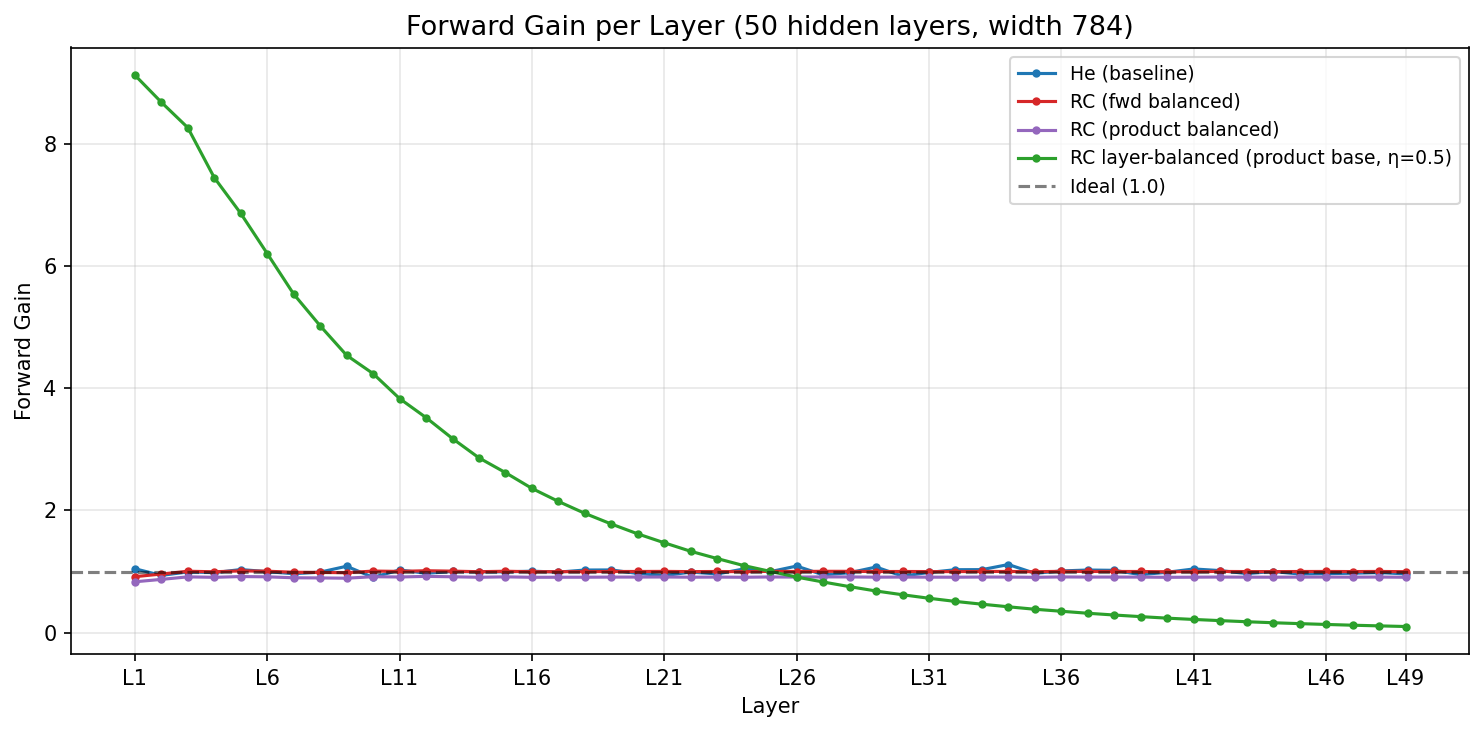
\includegraphics[width=0.92\textwidth]{forward_gain.png}
  \caption{Forward gain per layer.  He (blue) fluctuates around~1.0.
           Fwd-balanced (red) sits precisely at~1.0.
           Product-balanced (purple) sits at $\approx 0.91$.}
  \label{fig:fwd-gain}
\end{figure}

\subsection{Backward gain per layer}
\begin{figure}[H]
  \centering
  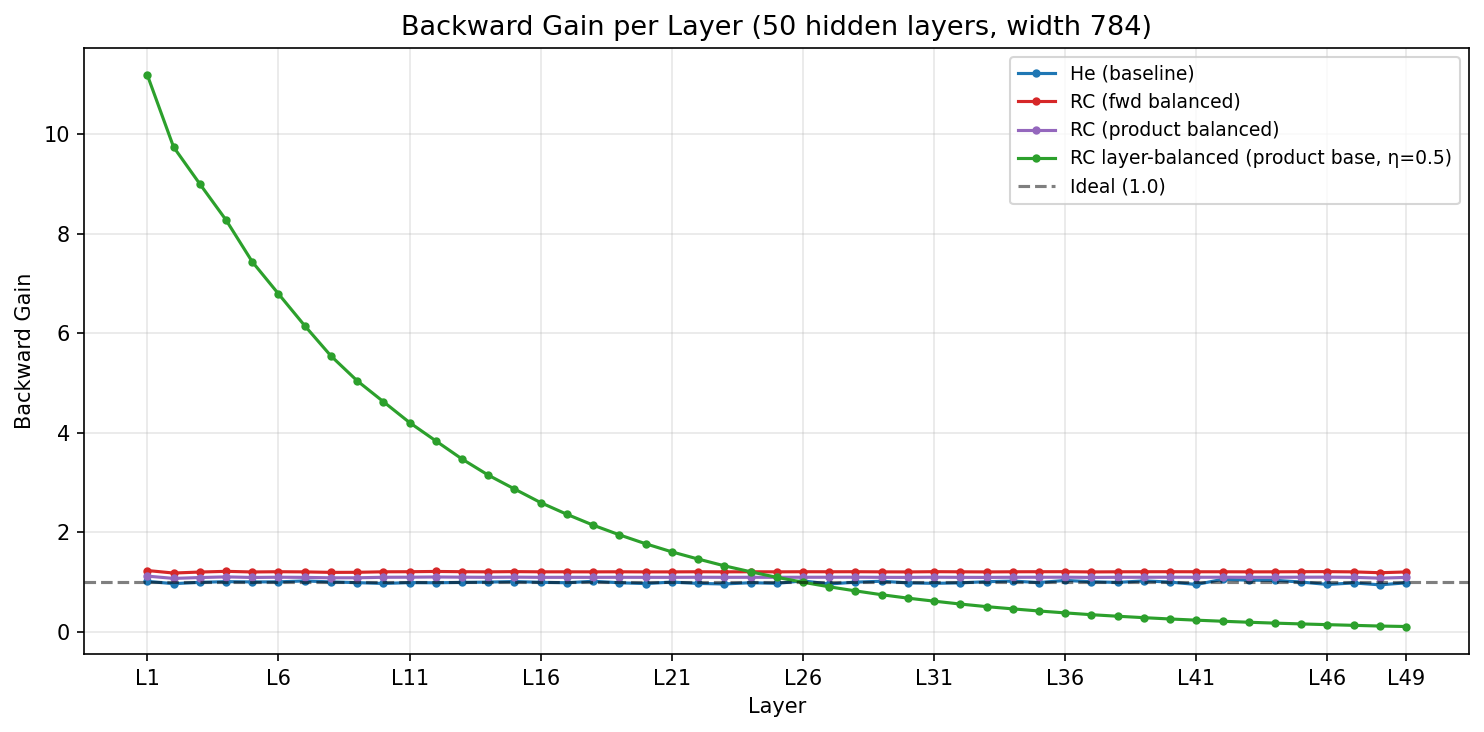
\includegraphics[width=0.92\textwidth]{backward_gain.png}
  \caption{Backward gain per layer.  He (blue) fluctuates around~1.0.
           Product-balanced (purple) sits at $\approx 1.10$.
           Fwd-balanced (red) is elevated at $\approx 1.21$.}
  \label{fig:bwd-gain}
\end{figure}

\subsection{Gain product per layer}
\begin{figure}[H]
  \centering
  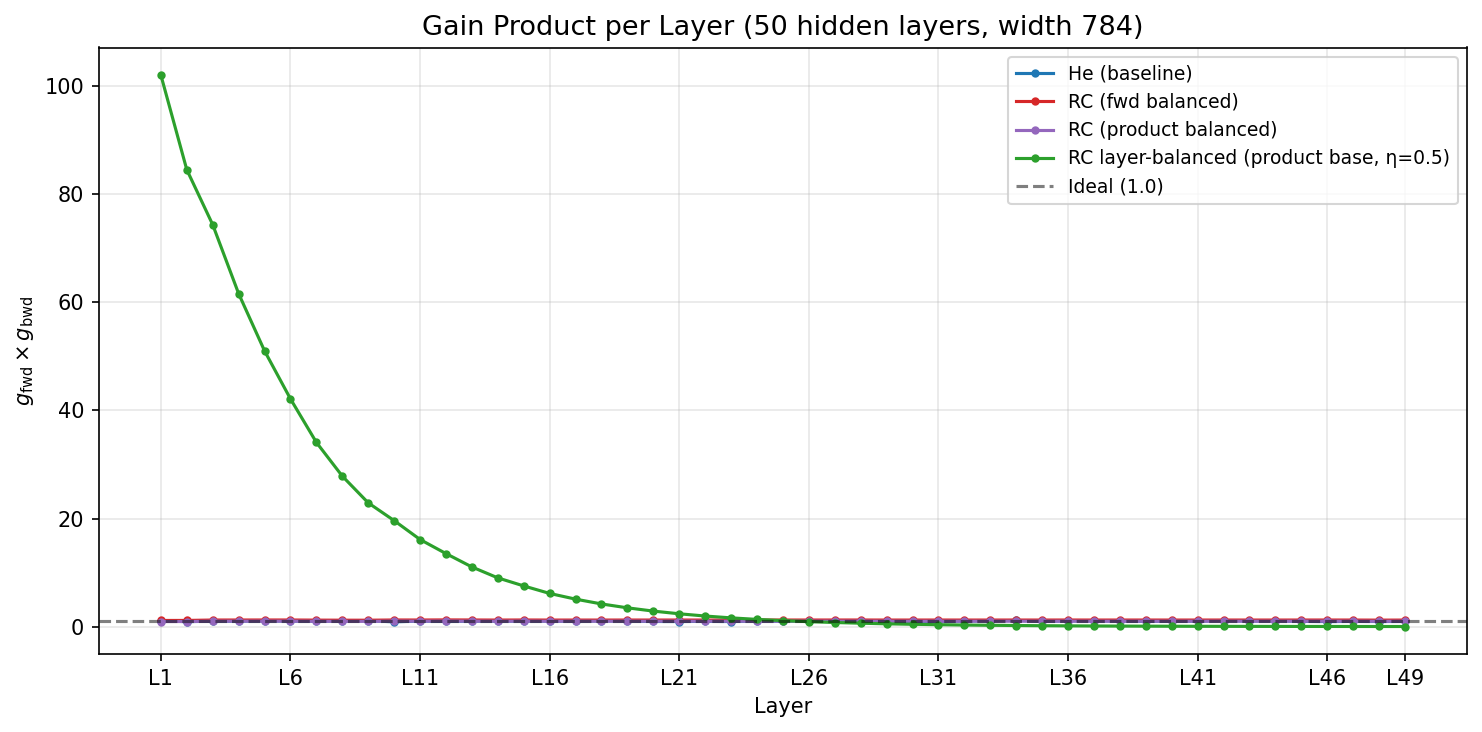
\includegraphics[width=0.92\textwidth]{gain_product.png}
  \caption{Gain product $g_{\mathrm{fwd}} \times g_{\mathrm{bwd}}$
           per layer.  \textbf{Product-balanced sits exactly at~1.0}
           (the design target).  He sits near~1.0 (both gains individually
           $\approx 1$).  Fwd-balanced sits at $\approx 1.21$ (product $> 1$).}
  \label{fig:gain-product}
\end{figure}


%======================================================================
\section{Geometry Preservation (k-NN Accuracy)}
\label{sec:geometry}

\subsection{Setup}
Fashion-MNIST, 2000 samples, depths $L \in \{5, 10, 15, 20\}$,
square projections (width = 784).  The k-NN accuracy ($k=5$)
measures whether class structure survives the multi-layer
projection.

\subsection{Results}

\begin{table}[H]
\centering
\caption{k-NN accuracy vs.\ depth.  Chance level = 0.10 (10 classes).}
\label{tab:knn}
\begin{tabular}{l c c c c}
\toprule
Initializer & 5\,L & 10\,L & 15\,L & 20\,L \\
\midrule
He (baseline)          & 0.829 & 0.800 & 0.784 & \textbf{0.752} \\
RC fwd-balanced        & 0.810 & 0.636 & 0.356 & 0.270 \\
RC product-balanced    & 0.810 & 0.636 & 0.356 & 0.269 \\
\bottomrule
\end{tabular}
\end{table}

\begin{figure}[H]
  \centering
  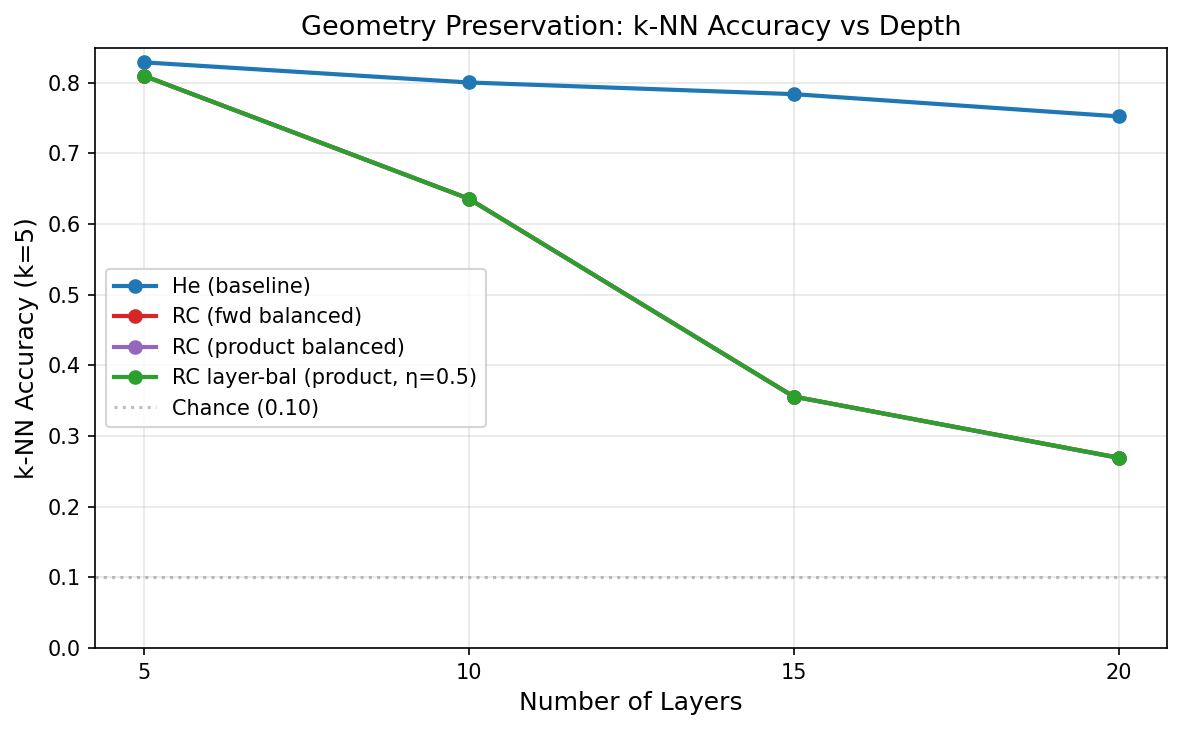
\includegraphics[width=0.7\textwidth]{knn_accuracy.png}
  \caption{k-NN accuracy vs.\ depth.  He degrades gracefully
           ($0.83 \to 0.75$).  Both RC variants collapse
           identically to~0.27 by 20 layers.}
  \label{fig:knn}
\end{figure}

\begin{remark}
  Product-balanced and fwd-balanced produce identical k-NN curves
  at every depth.  Both are fully row-centered ($\sum_j W_{ij} = 0$),
  so the DC-blindness --- the mechanism that destroys class structure
  (see main report, Chapter~5) --- is identical regardless of variance.
  Changing $s$ affects gain magnitudes but not the structural constraint.
\end{remark}


%======================================================================
\section{Per-Layer Variance Scaling: The $\eta$-Schedule}
\label{sec:layer-balanced}

Since uniform variance cannot produce uniform gradients, we
derive a per-layer variance schedule from BP4.

\subsection{Derivation from BP4}

\textbf{Step 1: Forward chain.}  Using \eqref{eq:fwd-gain}, the
activation RMS at layer~$\ell-1$ is:
\begin{equation}\label{eq:fwd-chain}
  \rms(A^{(\ell-1)})
  = \rms(A^{(0)}) \cdot \prod_{k=1}^{\ell-1} g_{\mathrm{fwd}}^{(k)}
  = \rms(A^{(0)}) \cdot \prod_{k=1}^{\ell-1} (r \cdot s_k)
  = \rms(A^{(0)}) \cdot r^{\ell-1} \cdot \prod_{k=1}^{\ell-1} s_k.
\end{equation}

\textbf{Step 2: Backward chain.}  The backward gain at position~$k$
is produced by the weight matrix $W^{(k+1)}$, so
$g_{\mathrm{bwd}}^{(k)} \approx s_{k+1}$.  Telescoping from
layer~$L$ down to layer~$\ell$:
\begin{equation}\label{eq:bwd-chain}
  \rms(\Delta^{(\ell)})
  = \rms(\Delta^{(L)}) \cdot \prod_{k=\ell}^{L-1} g_{\mathrm{bwd}}^{(k)}
  = \rms(\Delta^{(L)}) \cdot \prod_{k=\ell+1}^{L} s_k.
\end{equation}

\textbf{Step 3: Gradient at layer~$\ell$.}  Substituting
\eqref{eq:fwd-chain} and \eqref{eq:bwd-chain} into \eqref{eq:grad-mag}:
\begin{align}
  \left\|\frac{\partial\mathcal{C}}{\partial W^{(\ell)}}\right\|
  &\propto r^{\ell-1} \cdot \prod_{k=1}^{\ell-1} s_k
           \cdot \prod_{k=\ell+1}^{L} s_k \notag \\
  &= r^{\ell-1} \cdot \frac{\prod_{k=1}^{L} s_k}{s_\ell}. \label{eq:gradient-formula}
\end{align}
Since $\prod_{k=1}^L s_k$ is a constant (independent of~$\ell$):
\begin{equation}\label{eq:gradient-simple}
  \boxed{\;\left\|\frac{\partial\mathcal{C}}{\partial W^{(\ell)}}\right\|
  \propto \frac{r^{\ell-1}}{s_\ell}.\;}
\end{equation}

\textbf{Step 4: Condition for uniform gradients.}
\begin{equation}\label{eq:uniform-condition}
  \frac{r^{\ell-1}}{s_\ell} = \text{const for all } \ell
  \quad\Longleftrightarrow\quad
  s_\ell \propto r^{\ell-1}.
\end{equation}

\subsection{The $\eta$-parameterization}

Rather than setting $s_\ell = C \cdot r^{\ell-1}$ directly (which
would fully correct the gradient at the cost of extreme variance
differences between layers), we introduce a \emph{correction strength}
parameter $\eta \in [0, 1]$:
\begin{equation}\label{eq:eta-schedule}
  s_\ell = s_{\mathrm{base}} \cdot r^{\,\eta\,(\ell - (L+1)/2)},
\end{equation}
where:
\begin{itemize}[nosep]
  \item $\ell \in \{1, \ldots, L\}$ is the 1-indexed layer number.
  \item $L$ is the total number of weight layers.
  \item The exponent is centered at the middle layer $\ell = (L+1)/2$,
        so the geometric mean of all $s_\ell$ equals $s_{\mathrm{base}}$.
  \item $s_{\mathrm{base}} = s^{\ast} = (\pi/(\pi-1))^{1/4}$ is the
        product-balanced factor from Section~\ref{sec:product-balanced}.
\end{itemize}

The parameter $\eta$ is \textbf{not derived from theory} --- it is a
tunable knob that controls the trade-off between gradient uniformity
and variance uniformity:
\begin{itemize}[nosep]
  \item $\eta = 0$: uniform variance ($s_\ell = s^{\ast}$ for all $\ell$).
        Gradient ratio $= r^{-(L-1)}$.  No correction.
  \item $\eta = 1$: full correction ($s_\ell \propto r^{\ell-1}$).
        Gradient ratio $= 1$ (perfect uniformity), but variance ratio
        $= r^{-(L-1)}$ (extreme).
  \item $0 < \eta < 1$: partial correction --- a compromise.
\end{itemize}

The per-layer weight standard deviation is then:
\begin{equation}\label{eq:target-std}
  \sigma_\ell = \sqrt{\frac{2}{d_{\ell-1}}} \cdot s_\ell
              = \sqrt{\frac{2}{d_{\ell-1}}} \cdot s^{\ast} \cdot r^{\,\eta\,(\ell - (L+1)/2)}.
\end{equation}

The initialization procedure is the same as
Definition~\ref{def:init-procedure}, but with $\sigma_\ell$
varying per layer.


%======================================================================
\section{The Pareto Frontier}
\label{sec:pareto}

\subsection{The fundamental trade-off}

\begin{theorem}[Pareto budget]
  \label{thm:pareto}
  For the $\eta$-schedule \eqref{eq:eta-schedule}, define:
  \begin{align}
    G(\eta) &= r^{-(1-\eta)(L-1)} \quad\text{(gradient ratio: max/min gradient)}, \label{eq:grad-ratio-formula} \\
    V(\eta) &= r^{-\eta(L-1)} \quad\text{(variance ratio: max/min weight std)}.  \label{eq:var-ratio-formula}
  \end{align}
  Then their product is independent of~$\eta$:
  \begin{equation}\label{eq:pareto}
    \boxed{\;G(\eta) \cdot V(\eta) = r^{-(L-1)}.\;}
  \end{equation}
\end{theorem}

\begin{proof}
  \begin{align*}
    G(\eta) \cdot V(\eta)
    &= r^{-(1-\eta)(L-1)} \cdot r^{-\eta(L-1)} \\
    &= r^{-\bigl[(1-\eta) + \eta\bigr](L-1)} \\
    &= r^{-(L-1)}.
  \end{align*}
\end{proof}

This means: reducing the gradient ratio by a factor of~$k$
necessarily \emph{increases} the variance ratio by the same
factor.  The total ``budget'' $r^{-(L-1)}$ is fixed.

\subsection{Numerical consequences}

\begin{table}[H]
\centering
\caption{Pareto budget at various depths.  The budget grows
         exponentially, making the trade-off increasingly severe.}
\label{tab:budget}
\begin{tabular}{c c}
\toprule
Depth $L$ & Budget $r^{-(L-1)}$ \\
\midrule
10  & $5.6\times$ \\
20  & $38\times$ \\
50  & $11{,}943\times$ \\
100 & $1.7 \times 10^8$ \\
\bottomrule
\end{tabular}
\end{table}

At $L = 20$, the budget is $38\times$ --- one can set $\eta = 0.75$
to get gradient ratio $\approx 2.5\times$ and variance ratio
$\approx 15\times$, both manageable.

At $L = 50$, the budget is $\sim\!12{,}000\times$.  Even the
``fairest'' split ($\eta = 0.5$, both factors $\approx 109\times$)
is severe.

\subsection{Depth-adaptive $\eta$}

Given a target gradient ratio~$T$, one can solve for the
required~$\eta$ from \eqref{eq:grad-ratio-formula}:
\begin{equation}\label{eq:eta-adaptive}
  \eta^{\ast}(L, T)
  = \max\!\left(0,\;\; 1 - \frac{\ln T}{(L-1) \cdot \ln(1/r)}\right).
\end{equation}

\begin{table}[H]
\centering
\caption{Depth-adaptive $\eta$ for target gradient ratio $T = 10\times$.}
\label{tab:adaptive}
\begin{tabular}{c c c c}
\toprule
$L$ & $\eta^{\ast}$ & Gradient ratio & Variance ratio \\
\midrule
10  & 0.000 & $5.6\times$  & $1.0\times$ \\
20  & 0.368 & $10\times$   & $3.8\times$ \\
50  & 0.755 & $10\times$   & $1{,}194\times$ \\
100 & 0.879 & $10\times$   & $17{,}276{,}021\times$ \\
\bottomrule
\end{tabular}
\end{table}

At $L = 50$, achieving gradient ratio $\leq 10\times$ requires
variance ratio $\geq 1{,}194\times$: the weight standard deviation
at the first layer would be $\sim\!38\times$ larger than at the
last layer.  While this is numerically representable in float32,
the extreme scale difference between layers creates practical
training difficulties (e.g., a single learning rate cannot
serve all layers well).

\subsection{Varying widths}
\label{sec:varying-width}

If $d_{\ell-1} \neq d_\ell$, equation~\eqref{eq:gradient-formula}
acquires an additional factor $\sqrt{d_\ell \cdot d_{\ell-1}}$:
\[
  \left\|\frac{\partial\mathcal{C}}{\partial W^{(\ell)}}\right\|
  \propto \sqrt{d_\ell \cdot d_{\ell-1}} \cdot \frac{r^{\ell-1}}{s_\ell}.
\]
The $\sqrt{d_\ell \cdot d_{\ell-1}}$ factor is layer-dependent
but can be absorbed into the per-layer scaling $s_\ell$.  The
fundamental Pareto structure (Theorem~\ref{thm:pareto}) is
unchanged: the $r^{\ell-1}$ term still requires non-uniform
$s_\ell$ to cancel, and the budget $r^{-(L-1)}$ remains.


%======================================================================
\section{Conclusion}
\label{sec:conclusion}

\subsection{Results}

\begin{enumerate}
  \item The product-balanced variance $v^{\ast} = 2\sqrt{\pi/(\pi-1)}/d
        \approx 2.422/d$ is the unique solution to
        $g_{\mathrm{fwd}} \cdot g_{\mathrm{bwd}} = 1$.
        Empirically verified to 0.2\% accuracy at 50 hidden layers.

  \item The Pareto budget theorem: for any row-centered per-layer
        schedule, $G(\eta) \cdot V(\eta) = r^{-(L-1)}$.  This budget
        grows exponentially with depth and cannot be reduced by any
        choice of~$\eta$.

  \item Geometry experiments (k-NN accuracy) confirm that \emph{all}
        row-centered variants --- regardless of variance --- produce
        identical geometry degradation.  The DC-blindness inherent to
        row centering is the mechanism, and it is unaffected by~$s$.
\end{enumerate}

\subsection{Implications}

For deep networks ($L \geq 50$):

\begin{itemize}
  \item \textbf{Gradient stability} within the row-centering framework
        requires a per-layer variance schedule, but the exponential
        Pareto budget makes this increasingly impractical with depth.
        Escaping the Pareto frontier requires abandoning the structural
        constraint $\sum_j W_{ij} = 0$ --- i.e., moving away from full
        row centering.

  \item \textbf{Geometry preservation} is impossible with row centering
        at depth.  The DC-blindness that defines row centering is the
        same mechanism that destroys class structure.

  \item The product-balanced initializer remains useful as an
        \textbf{analytical tool}: it identifies the midpoint of the
        gain space and provides the natural base for per-layer schemes
        at moderate depth ($L \leq 20$).
\end{itemize}

\end{document}
